In this problem, a function $u(x)$, defined on the unit interval $[0,1]$, is considered. The Poisson equation with a Neumann boundary condition
\begin{equation}\label{poisson}
    u_{xx} = f(x), \, u(0) = \alpha, \, u_x(1) = \sigma,
\end{equation}
will be solved analytically. Moreover, it will be solved numerically on a grid of equidistant points
\begin{equation*}
    x_0 = 0, \, x_1 = \frac{1}{M+1}, \, \dots, \, x_M = \frac{M}{M+1}, \, x_{M+1} = 1. 
\end{equation*}
A node on the $x$-axis will be denoted by $x_m=mh$ where $0 \leq m \leq M+1$ and the step length is $h = \frac{1}{M+1}$.

\subsubsection{a)}

Let $f(x) := \cos{(2\pi x)} + x$ and $\alpha = \sigma = 0$. The analytical solution to \eqref{poisson}, denoted by $u(x)$, is found by integrating twice, before applying the boundary conditions

\begin{equation*}
\begin{split}
    u_{xx} &= \cos{(2\pi x)} + x, \\
    u_x(x) &= \frac{1}{2\pi}\sin{(2\pi x)} + \frac12x^2 + C_1, \\
    u_x(1) &= \frac12 + C_1 = 0 \implies C_1 = -\frac12, \\
    u(x) &= -\frac{1}{4\pi^2}\cos{(2\pi x)} + \frac16x^3 + C_1x + C_2, \\
    u(0) &= -\frac{1}{4\pi^2} + C_2 = 0 \implies C_2 = \frac{1}{4\pi^2}, \\
    \implies u(x) &= -\frac{1}{4\pi^2}\cos{(2\pi x)} + \frac16x^3 -\frac12x + \frac{1}{4\pi^2}.
\end{split}
\end{equation*}
In order to approximate the analytical solution numerically, the linear system $A_h\boldsymbol{U} = \boldsymbol{f}$, with 
\begin{equation*}
    A_h = \frac{1}{h^2}\begin{pmatrix} 
    -2 & 1 & 0 & \dots & 0 \\
    1 & -2 & 1 & \ddots & 0 \\
    \ddots & \ddots & \ddots & \ddots & \ddots \\
    0 & \ddots & 1 & -2 & 1 \\
    0 & \dots & \frac h2 & -2h & \frac{3h}{2}
    \end{pmatrix}, \, 
    \boldsymbol{U} = \begin{pmatrix}
    U_1 \\
    U_2 \\
    \vdots \\
    U_M \\
    U_{M+1}
    \end{pmatrix}, \, \boldsymbol{f} = \begin{pmatrix}
    f(x_1) - \alpha/h^2 \\
    f(x_2) \\
    \vdots \\
    f(x_M) \\
    \sigma
    \end{pmatrix},
\end{equation*}
is constructed. Note that the numerical solution in each grid point $x_m$ is denoted by $U_m$. The central difference approximation
\begin{equation}
    u''_m = \frac{1}{h^2} \delta^2 u_m = \frac{1}{h^2}(u_{m-1} - 2u_m + u_{m+1}) + \mathcal{O}(h^2) = f_m \quad 1 \le m \le M,
    \label{centralDiff1a)}
\end{equation}
where $u_m := u(x_m)$ and $f_m := f(x_m)$, 
is used for all internal points on the grid. The truncation error for the central difference approximation is justified in section \ref{section_2.2}. For $x = 1$, the approximation used is

\begin{equation}
\label{Second-order-first-der-B.C}
    \frac{\frac{1}{2}u(x-2h)-2u(x-h)+\frac{3}{2}u(x)}{h} = u'(x) + \mathcal{O}(h^2). 
\end{equation}
It can be verified that this is a second order approximation of the first derivative by inserting the Taylor expansion up to third order for each term 

\begin{equation*}
    \begin{split}
        \frac{1}{2h}& \left\{u(x)-2hu'(x)+2h^2u''(x)-\frac{4h^3}{3}u^{(3)}(x) \right.\\
        &\left.-4\left(u(x) -hu'(x)+\frac{h^2}{2}u''(x)-\frac{h^3}{6}u^{(3)}(x)\right) + 3u(x) + \mathcal{O}(h^4)\right\} \\
        = &\frac{1}{2h}\left\{2h u'(x) - \frac{2h^3}{3}u^{(3)}(x)\right\} = u'(x) + \mathcal{O}(h^2).
    \end{split}
\end{equation*}
Inserting the numerical solution $U_{M+1}$ at $x_{M+1} = 1$ and neglecting the truncation error $\mathcal{O}(h^2)$ gives 

\begin{equation*}
    \frac{\frac{1}{2}U_{M-1}-2U_{M}+\frac{3}{2}U_{M+1}}{h} = \sigma, 
\end{equation*}
which coincides with the last row in the linear system above. This system is solved numerically via a linear equation solver in Python, which gives the approximate solution. Both the analytical and the numerical solutions are plotted in figure \ref{fig:part1Task1asolutions}. 

\begin{figure}
\centering
\subfloat[Analytical and numerical solution]{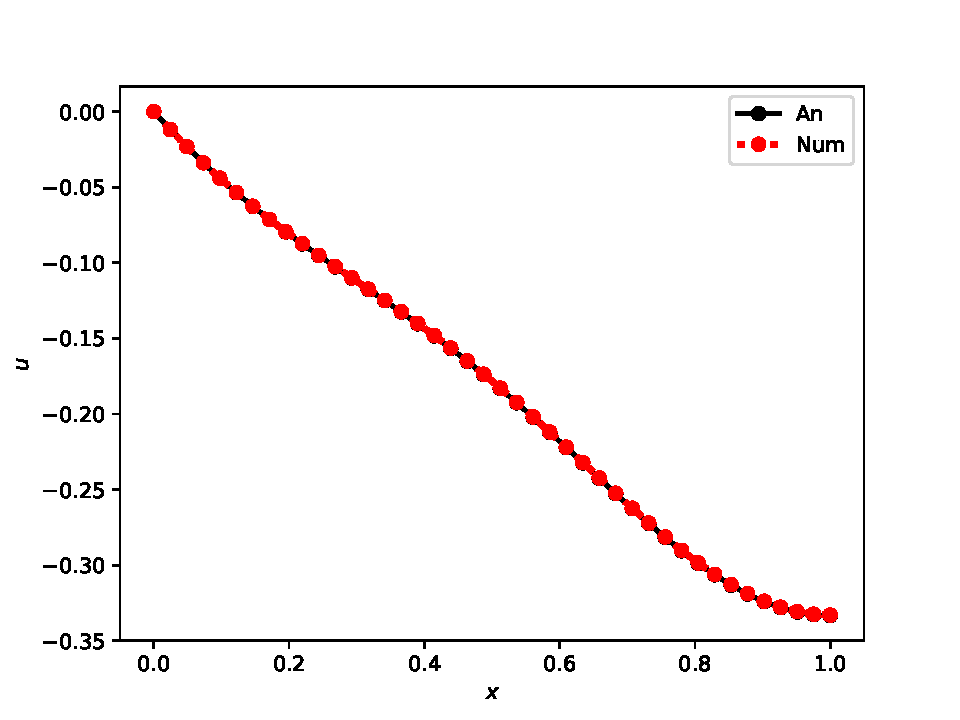
\includegraphics[width=0.85\linewidth]{plots/solutionsTask1a.pdf}\label{fig:part1Task1asolutions}}\hspace{0mm}
\subfloat[Relative error]{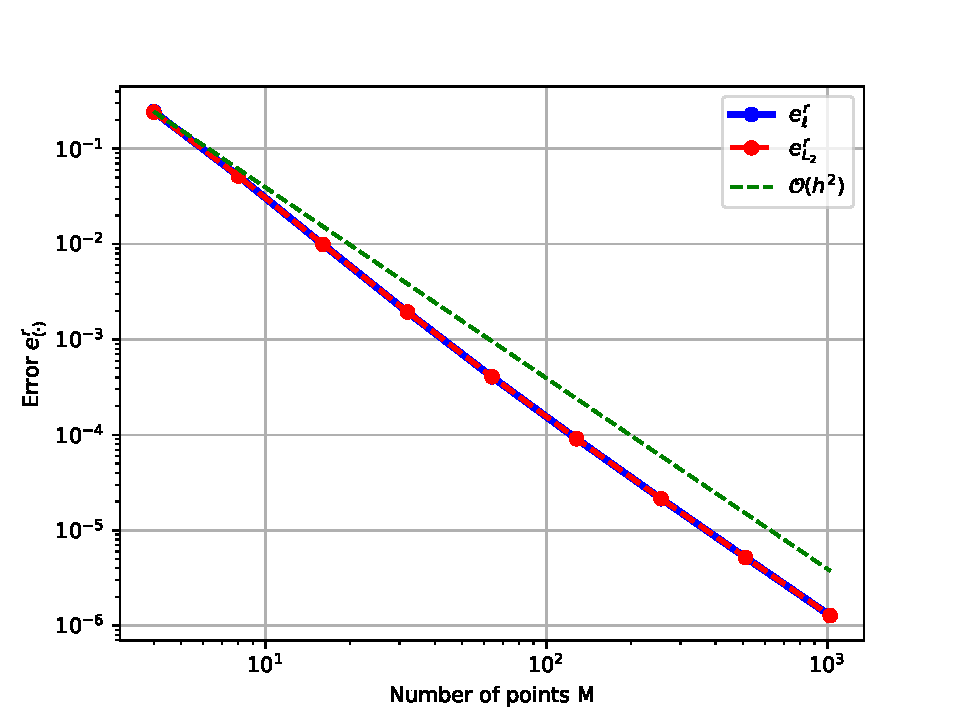
\includegraphics[width=0.85\linewidth]{plots/loglogtask1a.pdf}\label{fig:part1Task1aloglog}}\hspace{0mm}
\caption{Poisson equation with $f(x) := \cos{(2\pi x)} + x$, and boundary conditions $u(0) = 0$ and $u_x(1) = 0$. The analytical and numerical solution, solved and plotted on a grid with $M = 40$ points, is shown in (a). In (b), a "log-log" plot of relative errors when $h \rightarrow 0$ is shown.  $e^r_{L_2}$ is plotted with a dotted red line and $e^r_\ell$ is shown in blue. A green line of order $\mathcal{O}(h^2)$ is added to confirm the convergence order of the method. }
\end{figure}

In order to quantify the convergence of the numerical solution to the analytical solution, the relative errors $e_\ell^r$ and $e_{L_2}^r$, as defined in section \ref{errors.section}, are computed and plotted. 
A "$\log$-$\log$" plot of the relative errors in terms of increasing $M$ (decreasing $h \rightarrow 0$) are shown in figure \ref{fig:part1Task1aloglog}, i.e. $\log$-scales are used on both axes. The relative errors in both norms look very similar, and they show a convergence of order 2. This is, as shown, as expected. 
\newpage
\subsubsection{b)}    

A similar analysis is performed, but the boundary conditions are changed to two Dirichlet conditions

\begin{equation*}
    u(0) = 1, \, u(1) = 1.
\end{equation*}

\noindent In order to calculate the new analytical solution, a similar procedure as in part \textbf{a)} is followed. Thus, the analytical solution is given by 
\begin{equation*}
\begin{split}
    u_{xx} &= \cos{(2\pi x)} + x, \\
    u_x(x) &= \frac{1}{2\pi}\sin{(2\pi x)} + \frac12x^2 + C_1, \\
    u(x) &= -\frac{1}{4\pi^2}\cos{(2\pi x)} + \frac16x^3 + C_1x + C_2, \\
    u(0) &= -\frac{1}{4\pi^2} + C_2 = 1 \implies C_2 = 1+\frac{1}{4\pi^2}, \\
    u(1) &= -\frac{1}{4\pi^2} + \frac16 + C_1 + 1 + \frac{1}{4\pi^2} = 1 \implies C_1 = -\frac16, \\
    \implies u(x) &= -\frac{1}{4\pi^2}\cos{(2\pi x)} + \frac16x^3 -\frac16x + 1 + \frac{1}{4\pi^2}.
\end{split}
\end{equation*}
The linear system $A_h\boldsymbol{U} = \boldsymbol{f}$ is constructed, with 
\begin{equation*}
    A_h = \frac{1}{h^2}\begin{pmatrix} 
    -2 & 1 & 0 & \dots & 0 \\
    1 & -2 & 1 & \ddots & 0 \\
    \ddots & \ddots & \ddots & \ddots & \ddots \\
    0 & \ddots & 1 & -2 & 1 \\
    0 & \ddots & \ddots & 1 & -2
    \end{pmatrix}, \, 
    \boldsymbol{U} = \begin{pmatrix}
    U_1 \\
    U_2 \\
    \vdots \\
    U_M \\
    \end{pmatrix}, \, \boldsymbol{f} = \begin{pmatrix}
    f(x_1) - \frac{1}{h^2} \\
    f(x_2) \\
    \vdots \\
    f(x_M) - \frac{1}{h^2}\\
    \end{pmatrix}.
\end{equation*}
In this case, the central difference approximation \eqref{centralDiff1a)} is used for all points on the grid, except for the end points, where the function values are know. The analytical solution, as well as the numerical solution, is plotted in figure \ref{fig:part1Task1bsolutions}. Second order convergence is expected, because the central finite difference scheme has a local truncation error of order $\mathcal{O}(h^2)$. The "$\log$-$\log$" plot, shown in figure \ref{fig:part1Task1bloglog}, confirms that the convergence is of second order. 

\begin{figure}
\centering
\subfloat[Analytical and numerical solution]{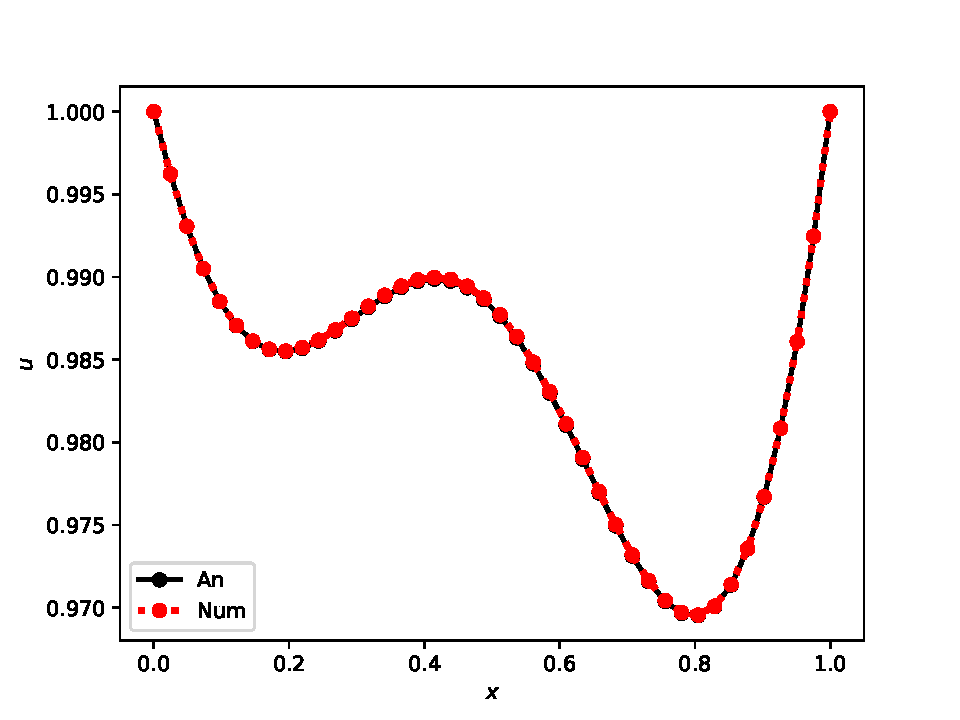
\includegraphics[width=0.85\linewidth]{plots/solutionsTask1b.pdf}\label{fig:part1Task1bsolutions}}\hspace{0mm}
\subfloat[Relative error]{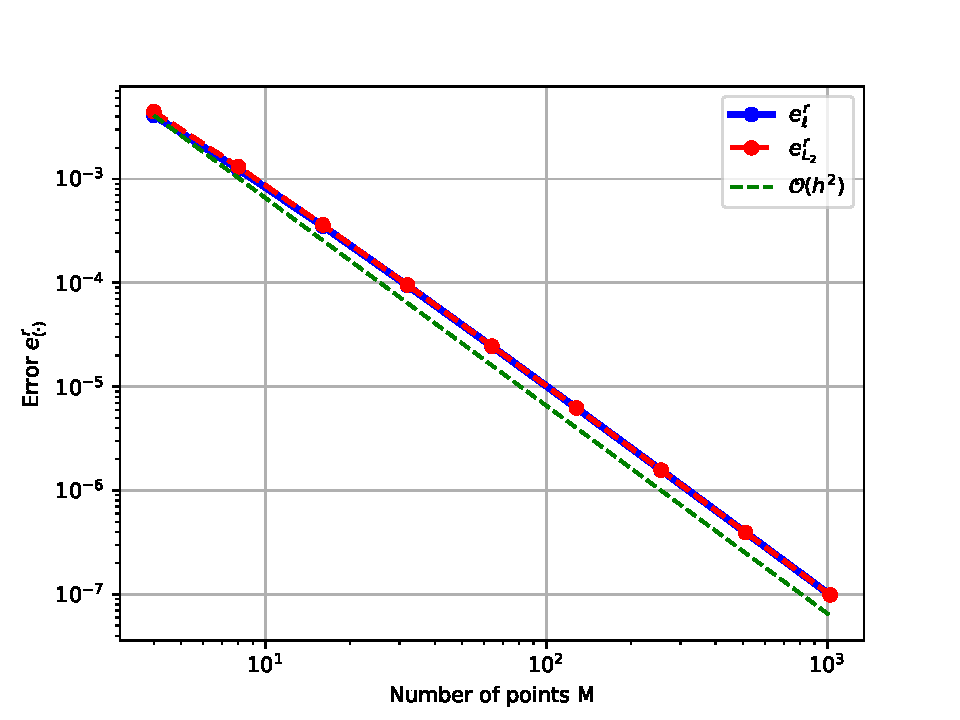
\includegraphics[width=0.85\linewidth]{plots/loglogtask1b.pdf}\label{fig:part1Task1bloglog}}\hspace{0mm}
\caption{Poisson equation with $f(x) := \cos{(2\pi x)} + x$, and boundary conditions $u(0) = 1$ and $u(1) = 1$. The analytical and numerical solution, solved and plotted on a grid with $M = 40$ points, is shown in (a). In (b), a "log-log" plot of relative errors when $h \rightarrow 0$ is shown. $e^r_{L_2}$ is plotted with a dotted red line and $e^r_\ell$ is shown in blue. A green line of order $\mathcal{O}(h^2)$ is added to confirm the convergence order of the method. }
\end{figure}

\subsubsection{c)}

The same problem is considered, but with two Neumann boundary conditions $u_x(0) = 0, \, u_x(1) = \frac{1}{2}$ instead. The issue with this specification is that the two Neumann conditions are the only conditions imposed, so the solution of the equation is ambiguous. The equation has either infinitely many solutions or zero solutions. This can be readily seen when solving the equation analytically, since there is one extra constant, $C_2$, that cannot be determined without imposing more conditions. A remedy could be to add a Dirichlet condition in at least one of the endpoints. In this way, one unambiguous solution can be determined down to the constant $C_2$. If this is done, the problem becomes very similar to the problem of task \textbf{a)}, and the numerical solution can be found in a similar manner. 

Another way to notice that the system is ambiguous is to consider a finite difference scheme with two fictitious nodes. A second order discretization of the Neumann boundary conditions using two fictitious external nodes $x_{-1}$ and $x_{M+2}$ is given by 
\begin{equation*}
    \frac{U_{1}-U_{-1}}{2h} = 0, \hspace{3mm} \frac{U_{M+2}-U_{M}}{2h} = \frac12.
\end{equation*}
These approximate boundary conditions lead to the elimination of the fictitious nodes $U_{-1} = U_1$ and $U_{M+2} = h + U_M$. Combining this with the second order central difference approximation \eqref{centralDiff1a)}, where the numerical solutions $U_m$ are inserted and the truncation error neglected, gives the equation for $m = 0$ 

\begin{comment}
    \begin{equation}
    \label{centralDifference}
        \frac{1}{h^2}(U_{m-1} - 2U_m + U_{m+1}) = f_m, \hspace{3mm} m = 0, \dots, M+1,
    \end{equation}
\end{comment}

\begin{equation*}
    \frac{U_1 - U_0}{h} = \frac{h}{2}f(x_0)
\end{equation*}
and the equation for $m = M+1$ 
\begin{equation*}
    \frac{U_M-U_{M+1}}{h} = \frac{h}{2}f(x_{M+1}) - \frac{1}{2}
\end{equation*}
Hence, the linear system takes the form

\begin{equation*}
    A_h = \frac{1}{h^2}\begin{pmatrix} 
    -h & h & 0 & \dots & 0 \\
    1 & -2 & 1 & \ddots & 0 \\
    \ddots & \ddots & \ddots & \ddots & \ddots \\
    0 & \ddots & 1 & -2 & 1 \\
    0 & \dots & \dots & h & -h
    \end{pmatrix}, \, 
    \boldsymbol{U} = \begin{pmatrix}
    U_0 \\
    U_1 \\
    \vdots \\
    U_{M+1} 
    \end{pmatrix}, \, \boldsymbol{f} = \begin{pmatrix}
    \frac{h}{2}f(x_0) \\
    f(x_1) \\
    \vdots \\
    \frac{h}{2}f(x_{M+1}) - \frac{1}{2}
    \end{pmatrix}.
\end{equation*}
It is apparent that the matrix $A_h$ is singular. Finally, the conclusion is that it cannot be solved.

\subsubsection{d)}

In this problem, the function $u(x) = \exp{\left(-\frac{1}{\epsilon}(x-\frac{1}{2})^2\right)}$ will be used as a manufactured solution for the boundary value problem 
\begin{equation}
    u_{xx} = f(x) \hspace{2mm} \text{in} \hspace{2mm} \Omega = (0,1),
\end{equation}
with Dirichlet boundary conditions $u(0) = \exp{\left(-\frac{1}{4\epsilon}\right)}$ and $u(1) = \exp{\left(-\frac{1}{4\epsilon}\right)}$. The constant $\epsilon$ determines the "steepness" of the curve, where the value $\epsilon = 0.01$ is used in our implementation. The function $f(x)$ can be calculated analytically from the manufactured solution

\begin{equation*}
\begin{split}
    f(x) &= \frac{\mathrm{d}^2}{\mathrm{d}x^2}\left(\exp{\left(-\frac{1}{\epsilon}\left(x-\frac{1}{2}\right)^2\right)}\right)\\ &= \frac{\mathrm{d}}{\mathrm{d}x}\left(-\frac{2}{\epsilon}\left(x-\frac{1}{2}\right)\exp{\left(-\frac{1}{\epsilon}\left(x-\frac{1}{2}\right)^2\right)}\right) \\
    &= -\frac{2}{\epsilon}\exp{\left(-\frac{1}{\epsilon}\left(x-\frac{1}{2}\right)^2\right)} + \frac{2}{\epsilon}\left(x-\frac{1}{2}\right)\frac{2}{\epsilon}\left(x-\frac{1}{2}\right)\exp{\left(-\frac{1}{\epsilon}\left(x-\frac{1}{2}\right)^2\right)} \\
    &= \frac{2}{\epsilon^2}\exp{\left(-\frac{1}{\epsilon}\left(x-\frac{1}{2}\right)^2\right)}\left(2\left(x-\frac{1}{2}\right)^2 -\epsilon \right).
\end{split}
\end{equation*}

How the numerical solutions converges to the manufactured solution is investigated for both second and first order methods using uniform mesh refinement (UMR) and adaptive mesh refinement (AMR).  

UMR will be used first, starting with the \textbf{first order method}. As seen from \eqref{Theory_approx_double_derivative} in section \ref{section_2.2}, applying the forward difference operator twice gives a first order approximation to the second derivative
\begin{equation*}
    \begin{split}
        &u_{xx}(x_m) = \frac{1}{h^2}\Delta^2u(x_m) + \mathcal{O}(h)\\
        \Rightarrow &f(x_m) = \frac{1}{h^2}(U_m-2U_{m+1}+U_{m+2}) \text{,} \hspace{2mm} 0 \leq m \leq M-1.
    \end{split}
\end{equation*}

\begin{comment}
\textcolor{red}{Old version;}
UMR will be used first, starting with the \textbf{first order method}. Applying the forward difference operator twice gives a first order approximation to the second derivative 
\begin{equation*}
\begin{split}
    u_{xx}(x_m) &= \frac{1}{h^2}\Delta^2u(x_m) + h\partial_x^3u(x_m) + \dots \\
    &= \frac{1}{h^2}\Delta(u(x_{m+1})-u(x_m)) + h\partial_x^3u(x_m) + \dots \\
    &= \frac{1}{h^2}(u(x_{m+2})-2u(x_{m+1}) + u(x_m)) + h\partial_x^3u(x_m) + \dots \\
    \implies
    f(x_i) &= \frac{1}{h^2}(U_i - 2U_{i+1} + U_{i+2}).
\end{split}
\end{equation*}
\textcolor{red}{Stop old version.}
\end{comment}

\noindent The implication follows from inserting the numerical approximation $U_m$ at each grid point $x_m$ and neglecting the truncation error $\mathcal{O}(h)$. 
\begin{figure}[t]
\centering
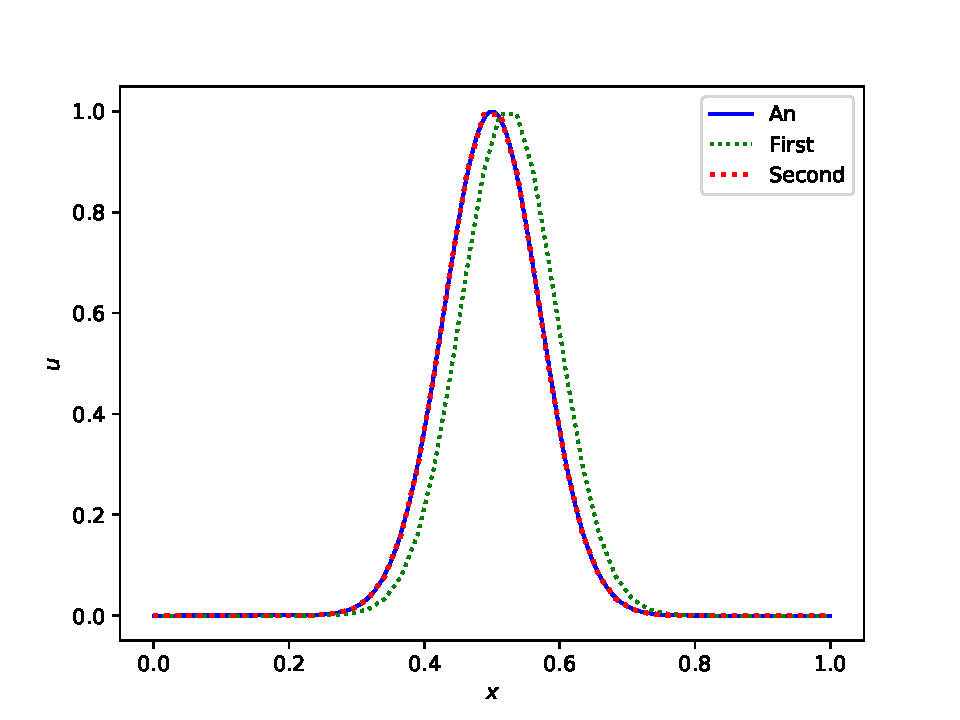
\includegraphics[width=0.85\linewidth]{plots/solutionTask1dUMR.pdf}
\caption{Poisson equation with manufactured solution $u(x) = \exp{\left(-\frac{1}{\epsilon}(x-\frac{1}{2})^2\right)}$, with Dirichlet boundary conditions $u(0) = u(1) = \exp{\left(-\frac{1}{4\epsilon}\right)}$. The manufactured solution, and numerical solutions solved with \textbf{UMR}, are plotted on a grid with $M = 40$ points. "First" refers to the solution using the first order method, while "Second" refers to the solution using the second order method.}
\label{fig:part1Task1dSolutionUMR}
\end{figure}
Adding the boundary conditions $U_0 = \alpha_1$ and $U_{M+1} = \alpha_2$ gives the linear system $A_h\boldsymbol{U} = \boldsymbol{f}$, with 

\begin{equation*}
    A_h = \frac{1}{h^2}\begin{pmatrix} 
    -2 & 1 & 0 & \dots & 0 \\
    1 & -2 & 1 & \ddots & 0 \\
    \ddots & \ddots & \ddots & \ddots & \ddots \\
    0 & \ddots & 1 & -2 & 1 \\
    0 & \dots & \dots & 1 & -2
    \end{pmatrix}, \, 
    \boldsymbol{U} = \begin{pmatrix}
    U_1 \\
    U_2 \\
    \vdots \\
    U_M 
    \end{pmatrix}, \, \boldsymbol{f} = \begin{pmatrix}
    f(x_0) - \alpha_1/h^2 \\
    f(x_1) \\
    \vdots \\
    f(x_{M-1}) - \alpha_2/h^2
    \end{pmatrix}.
\end{equation*}

The \textbf{second order method} is 

\begin{equation*}
    A_h = \frac{1}{h^2}\begin{pmatrix} 
    -2 & 1 & 0 & \dots & 0 \\
    1 & -2 & 1 & \ddots & 0 \\
    \ddots & \ddots & \ddots & \ddots & \ddots \\
    0 & \ddots & 1 & -2 & 1 \\
    0 & \dots & \dots & 1 & -2
    \end{pmatrix}, \, 
    \boldsymbol{U} = \begin{pmatrix}
    U_1 \\
    U_2 \\
    \vdots \\
    U_M 
    \end{pmatrix}, \, \boldsymbol{f} = \begin{pmatrix}
    f(x_1) - \alpha_1/h^2 \\
    f(x_2) \\
    \vdots \\
    f(x_M) - \alpha_2/h^2
    \end{pmatrix},
\end{equation*}

\noindent where a central difference scheme, as in equation \eqref{centralDiff1a)}, is used. The manufactured solution and numerical solutions when using both first and second order methods with UMR are shown in figure \ref{fig:part1Task1dSolutionUMR}. A "$\log$-$\log$" plot of the relative errors when using both first and second order methods with UMR are shown in figure \ref{fig:part1Task1dloglogUMR}. It is apparent that the convergence orders obtained in practice match the expected theoretical convergence orders for both schemes. These expectations are based on the $\mathcal{O}(h)$ truncation error of the first order method and the $\mathcal{O}(h^2)$ truncation error of the second order method.\newline


\begin{figure}
\centering
\subfloat[]{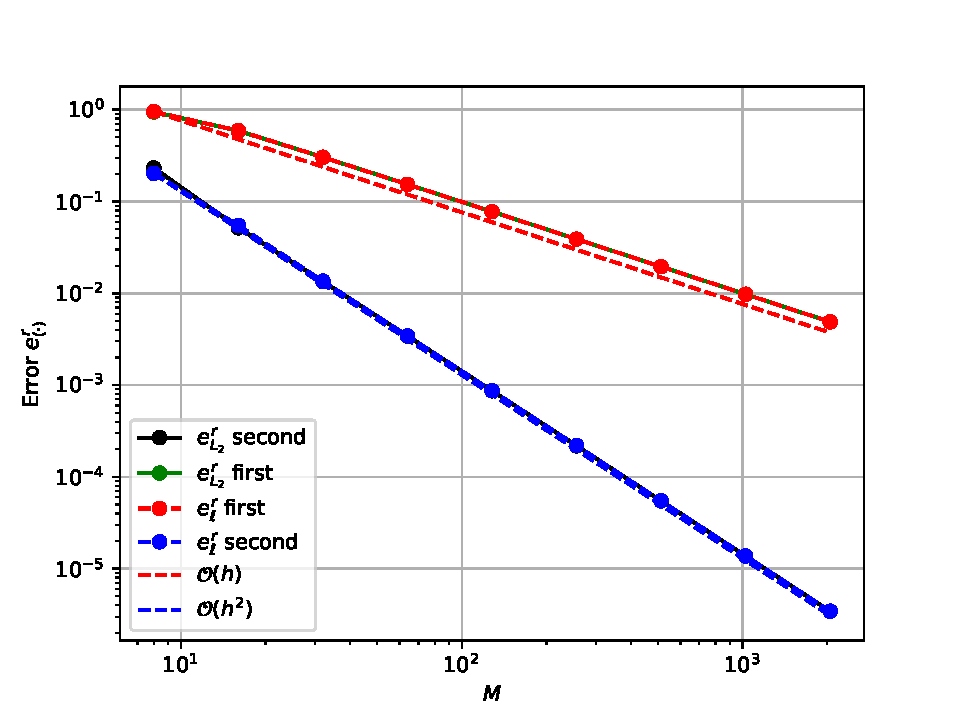
\includegraphics[width=0.85\linewidth]{plots/1d_UMR.pdf}\label{fig:part1Task1dloglogUMR}}\hspace{0mm}
\subfloat[]{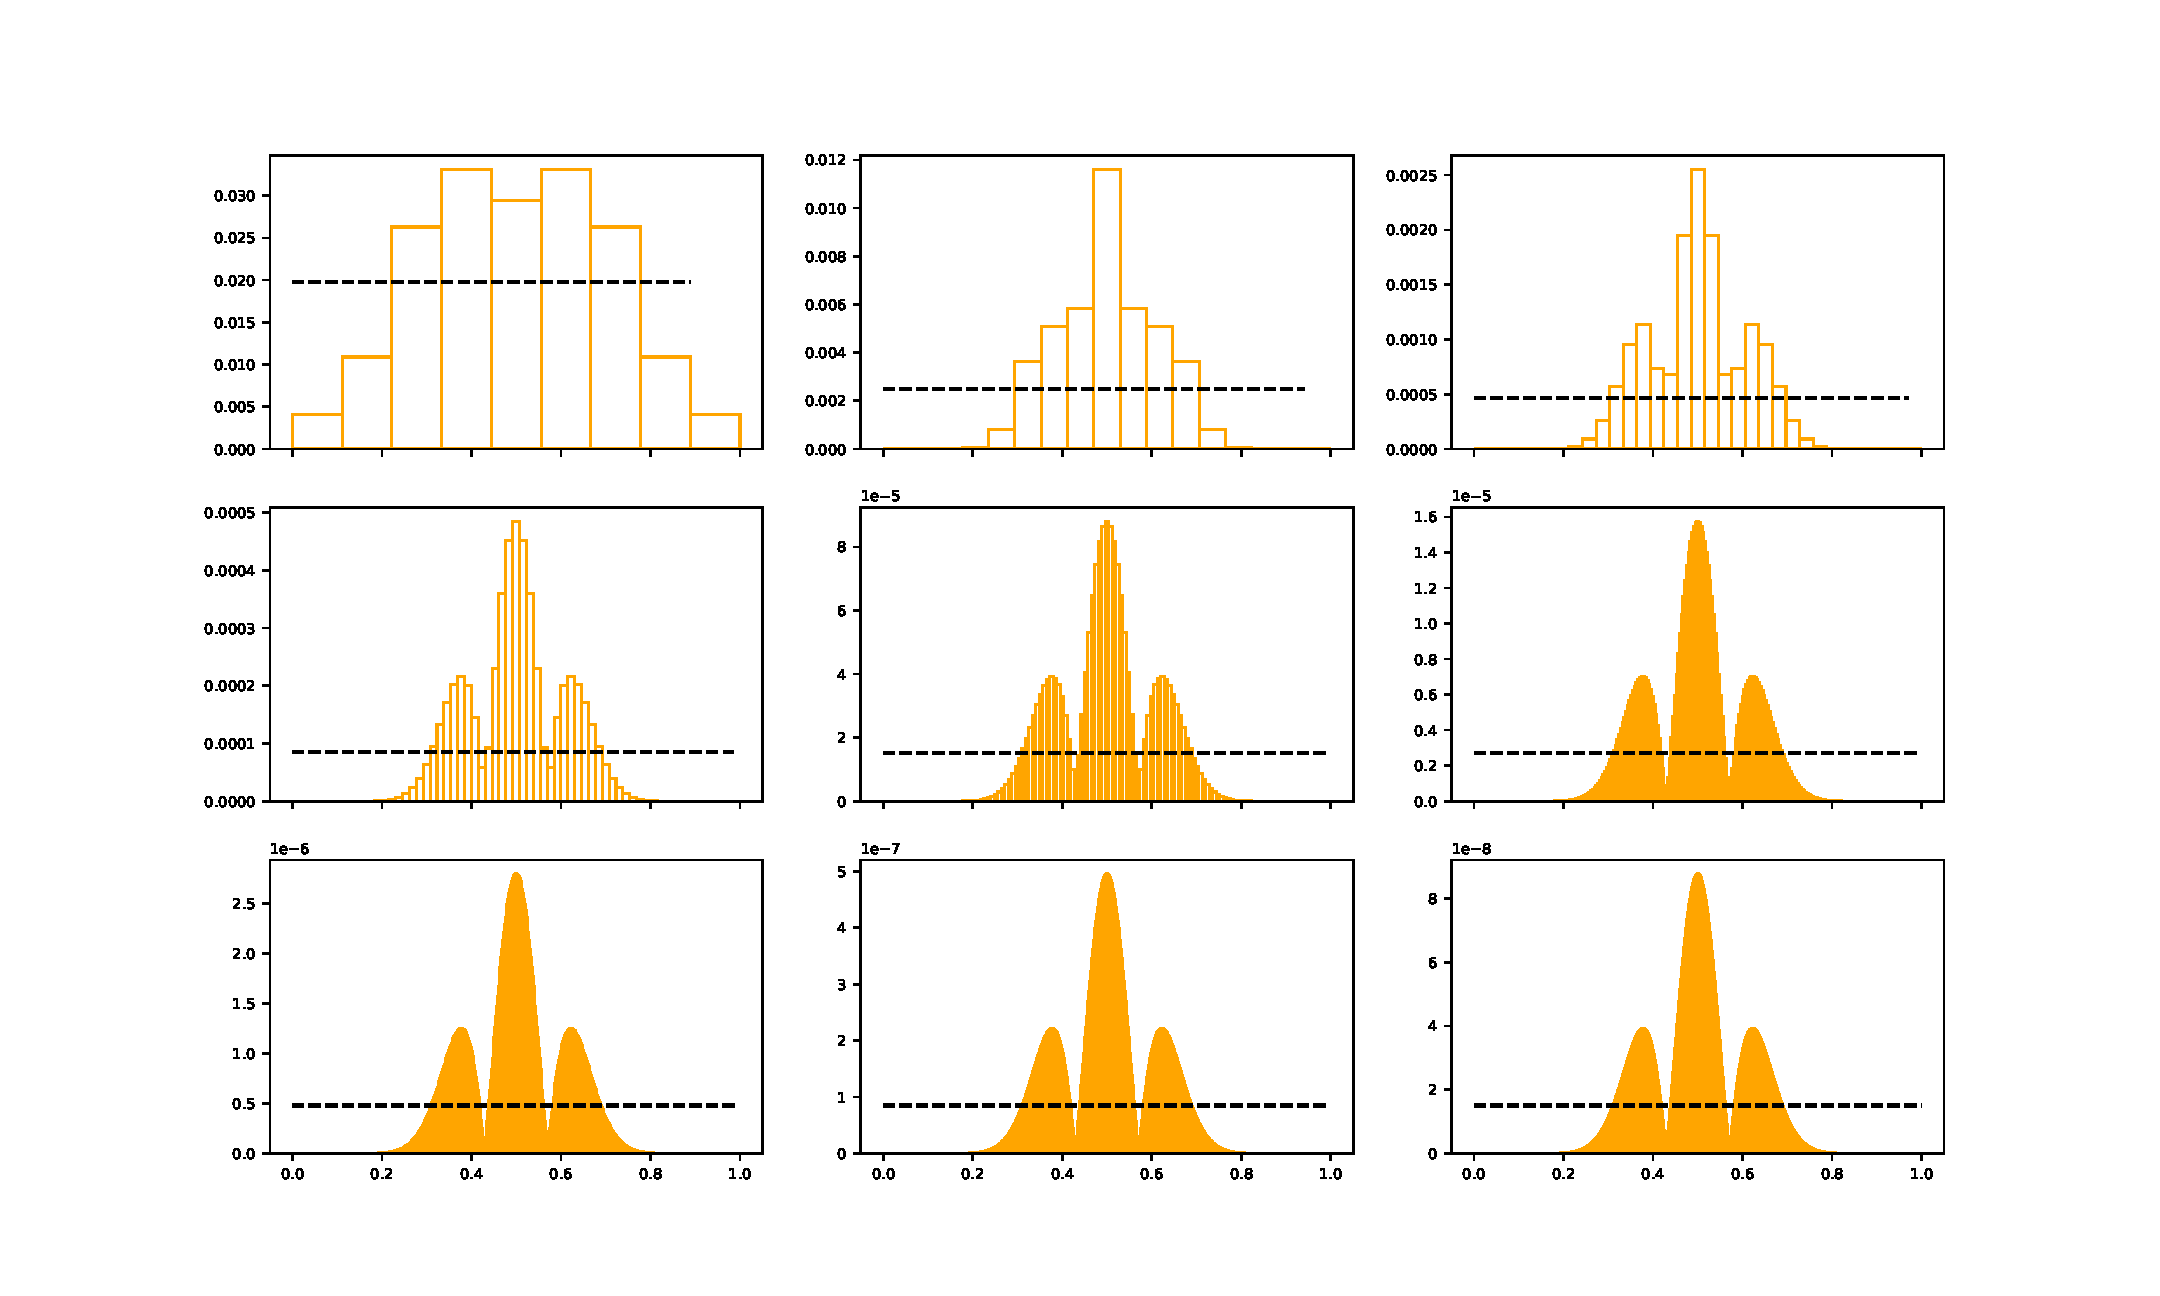
\includegraphics[width=0.85\linewidth]{plots/1d_UMR_barplot.pdf}\label{1d_UMR_barplot}}\hspace{0mm}

\caption{Poisson equation with manufactured solution $u(x) = \exp{\left(-\frac{1}{\epsilon}(x-\frac{1}{2})^2\right)}$, with Dirichlet boundary conditions $u(0) = u(1) = \exp{\left(-\frac{1}{4\epsilon}\right)}$. (a) A "log-log" plot of relative errors when $h \rightarrow 0$, when solving the problem using \textbf{UMR}, is shown. First and second order functions are added in order to compare to the convergence graphs of the numerical solutions. (b) A bar plot of the error associated with the second order solution on each sub-interval is shown. The dashed line indicates the average error. }
\end{figure}


In order to solve the boundary value problem using AMR, first and second order methods where the coefficients are dependent on the local step size need to be constructed. Liu et al. (1995) present stencils for methods of both orders in the article \textit{A high-resolution finite-difference scheme for nonuniform grids} \cite{Liu}. These are shown below. The implementation of AMR uses the average of the discrete error as the criterion for refinement. The error on each sub-interval of the grid, $I_i$ is modeled as a step-wise constant function, where the error is derived from the left end point of the interval. This means that the interval $I_i$ is split in two if

\textcolor{red}{Alt dette stemmer kanskje ikke overens med koden lenger?}
\begin{equation*}
    |u_i - U_i| \geq \frac{|u_1-U_1| + |u_2-U_2| + \dots + |u_{M-1} - U_N|}{N},
\end{equation*}
where $N$ is the number of sub-intervals at the current iteration and $u_i, U_i$ are the exact and approximate solutions at the left end-point of the $i$'th sub-interval, respectively.

A \textbf{first order method} with AMR is given by the three point stencil \cite{Liu}

\begin{equation*}
    (U_{xx})_m = bU_{m-1} - (b+c)U_{m} + cU_{m+1},
\end{equation*}
where the coefficients are given as 
\begin{equation*}
\begin{split}
    b = \frac{2}{h_{m-1}(h_{m-1}+h_{m})}, \\
    c = \frac{2}{h_{m}(h_{m-1}+h_{m})}, \\
    h_m = x_{m+1} - x_m.
\end{split}
\end{equation*}
With the Dirichlet boundary conditions, the system of equations becomes
\begin{equation*}
\begin{split}
    A_h &= \begin{pmatrix} 
    -(b+c) & c & 0 & \dots & 0 \\
    b & -(b+c) & c & \ddots & 0 \\
    \ddots & \ddots & \ddots & \ddots & \ddots \\
    0 & \ddots & b & -(b+c) & c \\
    0 & \dots & \dots & b & -(b+c)
    \end{pmatrix}, \\ 
    \boldsymbol{U} &= \begin{pmatrix}
    U_1 \\
    U_2 \\
    \vdots \\
    U_M 
    \end{pmatrix}, \, \boldsymbol{f} = \begin{pmatrix}
    f(x_1) - b\alpha_1 \\
    f(x_2) \\
    \vdots \\
    f(x_M) - c\alpha_2
    \end{pmatrix}.
\end{split}
\end{equation*}

A \textbf{second order method} with AMR is given by the four point stencil \cite{Liu}
\begin{equation}
\label{4_point_stencil}
    (U_{xx})_m = aU_{m-2} + bU_{m-1} - (a+b+c)U_m + cU_{m+1}
\end{equation}
where the coefficients are defined as
\begin{equation*}
\begin{split}
    a &= \frac{2(d_{m+1}-d_{m-1})}{d_{m-2}(d_{m-2}+d_{m+1})(d_{m-2}-d_{m-1})} \\
    b &= \frac{2(d_{m-2}-d_{m+1})}{d_{m-1}(d_{m-2}-d_{m-1})(d_{m-1}+d_{m+1})} \\
    c &= \frac{2(d_{m-2}+d_{m-1})}{d_{m+1}(d_{m-1}+d_{m+1})(d_{m-2}+d_{m+1})} \\
    d_{m+1} &=h_m, \hspace{2mm} d_{m-1} =h_{m-1}, \hspace{2mm} d_{m-2}=h_{m-2} + h_{m-1} \\ 
    h_m &= x_{m+1} - x_m.
\end{split}
\end{equation*}
By including the boundary conditions, the complete difference scheme becomes
\begin{equation*}
\begin{split}
    A_h &= \begin{pmatrix} 
    -(a+b+c) & c & 0 & \dots & \dots & 0 \\
    b & -(a+b+c) & c & \ddots & \ddots & 0 \\
    a & b & -(a+b+c) & c & \ddots & \vdots \\
    \ddots & \ddots & \ddots & \ddots & \ddots & \vdots\\
    0 & \ddots & a & b & -(a+b+c) & c \\
    0 & \dots & 0 & a & b & -(a+b+c)
    \end{pmatrix}, \, \\
    \boldsymbol{U} &= \begin{pmatrix}
    U_1 \\
    U_2 \\
    U_3 \\
    \vdots \\
    U_M 
    \end{pmatrix}, \, \hspace{2mm} \boldsymbol{f} = \begin{pmatrix}
    f(x_1) - b\alpha_1 \\
    f(x_2) - a\alpha_1\\
    f(x_3) \\
    \vdots \\
    f(x_M) - c\alpha_2
    \end{pmatrix}.
\end{split}
\end{equation*}

\begin{comment} % Vurdere hvilken som ser best ut
\begin{figure}[t]
  \centering
  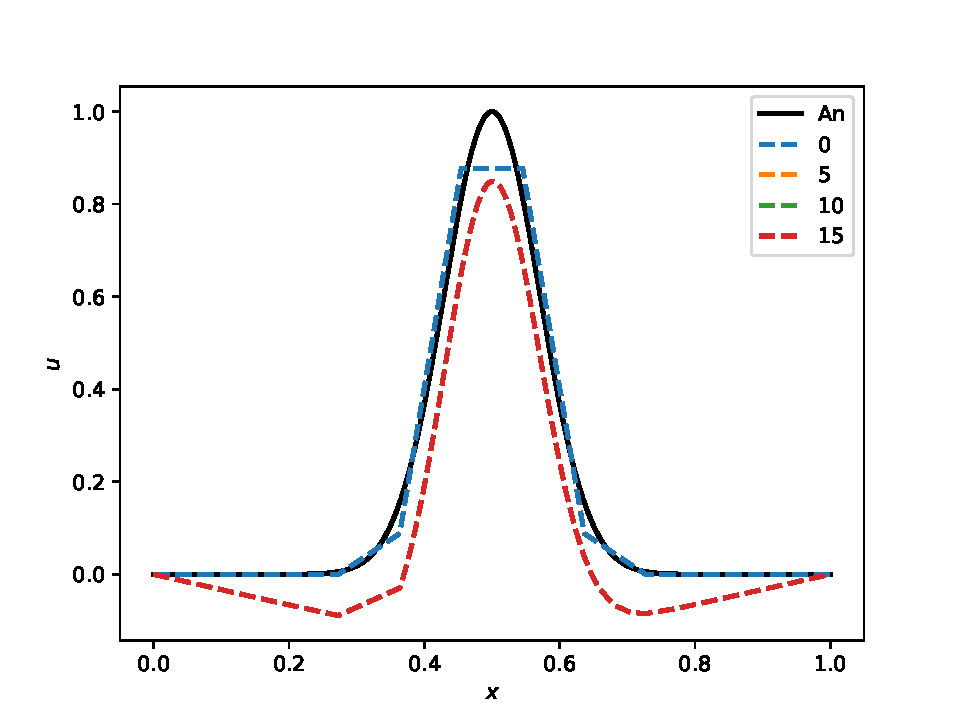
\includegraphics[width=.85\linewidth]{plots/solutionTask1dAMRFirst.pdf}
  \caption{Poisson equation with manufactured solution $u(x) = \exp{\left(-\frac{1}{\epsilon}(x-\frac{1}{2})^2\right)}$, with Dirichlet boundary conditions $u(0) = u(1) = \exp{\left(-\frac{1}{4\epsilon}\right)}$. Manufactured solution, and numerical solution solved with \textbf{AMR} and the \textbf{first order method}, plotted on a starting grid of $M = 10$ points. The grid is refined 7 times, where the integers in the legend refers to the numerical solution after each of the refinements.}

  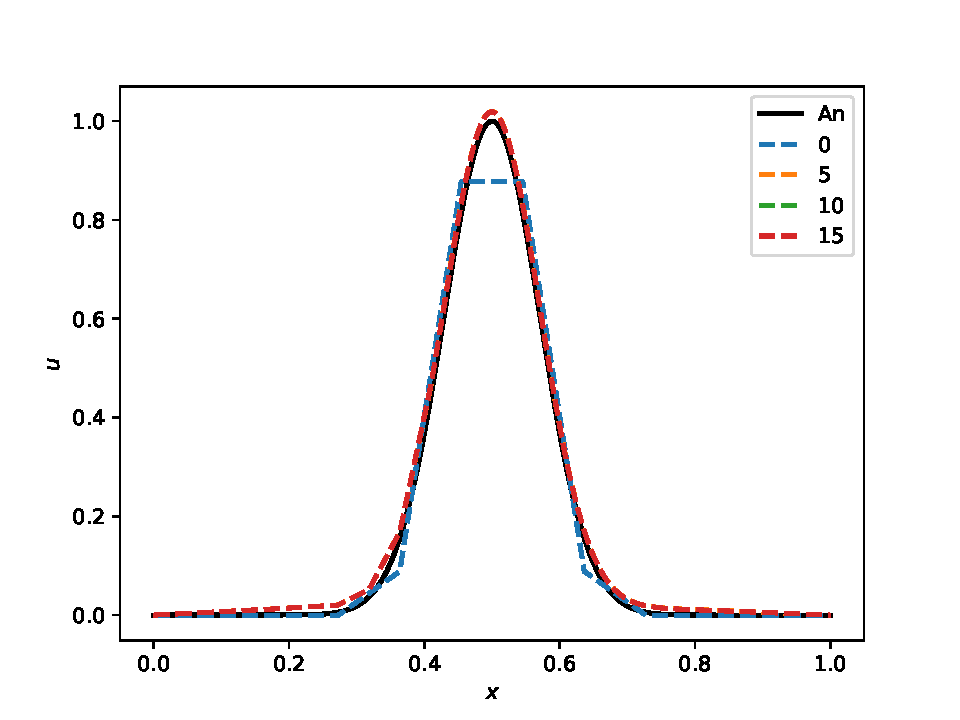
\includegraphics[width=.85\linewidth]{plots/solutionTask1dAMRSecond.pdf}
  \caption{Poisson equation with manufactured solution $u(x) = \exp{\left(-\frac{1}{\epsilon}(x-\frac{1}{2})^2\right)}$, with Dirichlet boundary conditions $u(0) = u(1) = \exp{\left(-\frac{1}{4\epsilon}\right)}$. Manufactured solution, and numerical solution solved with \textbf{AMR} and the \textbf{second order method}, plotted on a starting grid of $M = 10$ points. The grid is refined 7 times, where the integers in the legend refers to the numerical solution after each of the refinements.}
\end{figure}
\end{comment}

\begin{comment}
\begin{figure}[t]
\centering
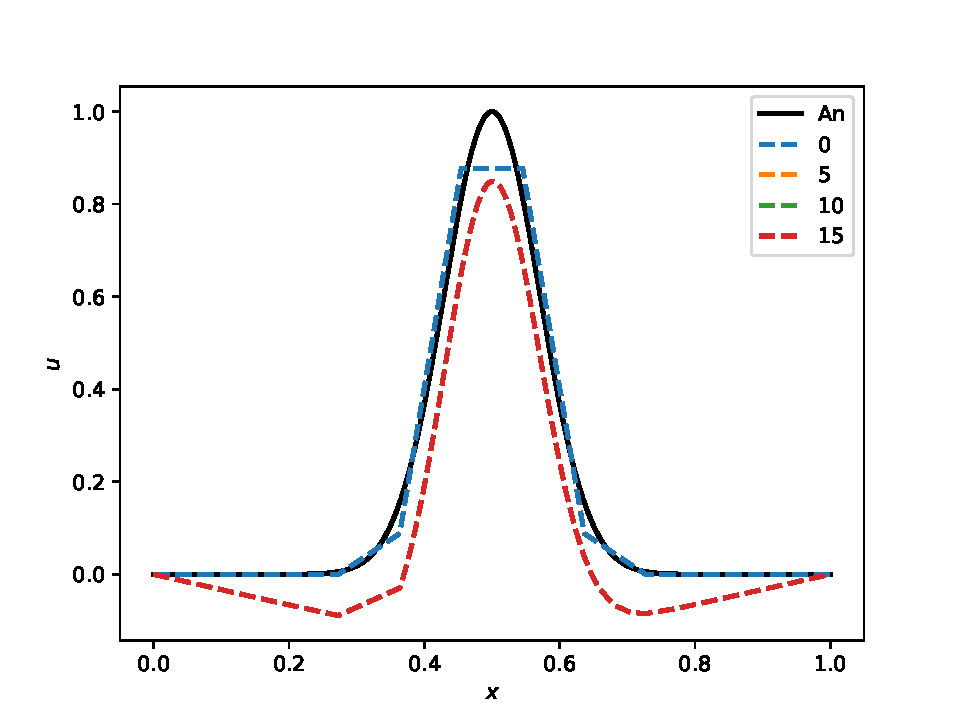
\includegraphics[width=\linewidth]{plots/solutionTask1dAMRFirst.pdf}
\caption{Poisson equation with manufactured solution $u(x) = \exp{\left(-\frac{1}{\epsilon}(x-\frac{1}{2})^2\right)}$, with Dirichlet boundary conditions $u(0) = u(1) = \exp{\left(-\frac{1}{4\epsilon}\right)}$. Manufactured solution, and numerical solution solved with \textbf{AMR} and the \textbf{first order method}, plotted on a starting grid of $M = 10$ points. The grid is refined 7 times, where the integers in the legend refers to the numerical solution after each of the refinements.}
\label{fig:part1Task1dSolutionAMRFirst}
\end{figure}

\begin{figure}[t]
\centering
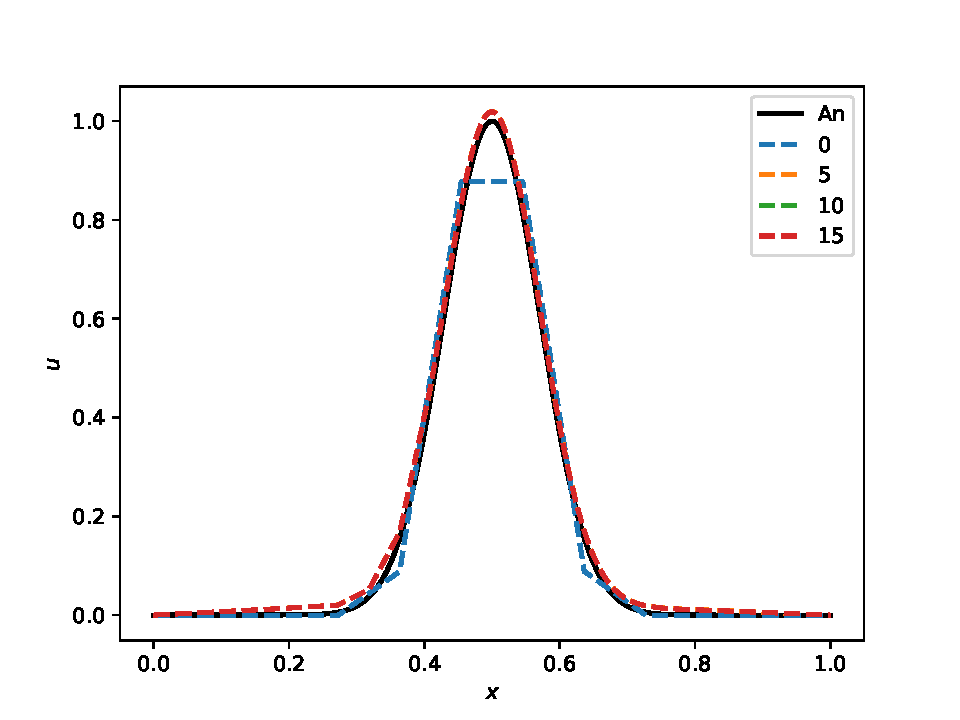
\includegraphics[width=\linewidth]{plots/solutionTask1dAMRSecond.pdf}
\caption{Poisson equation with manufactured solution $u(x) = \exp{\left(-\frac{1}{\epsilon}(x-\frac{1}{2})^2\right)}$, with Dirichlet boundary conditions $u(0) = u(1) = \exp{\left(-\frac{1}{4\epsilon}\right)}$. Manufactured solution, and numerical solution solved with \textbf{AMR} and the \textbf{second order method}, plotted on a starting grid of $M = 10$ points. The grid is refined 7 times, where the integers in the legend refers to the numerical solution after each of the refinements.}
\label{fig:part1Task1dSolutionAMRSecond}
\end{figure}
\end{comment}

We remark that for $m=1$ in equation \eqref{4_point_stencil}, the fictitious node $U_{-1}$ becomes an unknown in the linear system. To fix this, we immediately set $a_1 = 0$, by ensuring that $h_0 = h_1$ for the first two intervals. Hence, the fictitious node $U_{-1}$ is eliminated from the equation and the first equation in the linear system yields $(U_{xx})_1=\frac{1}{h_0^2}(U_0-2U_1+U_2)$. This equation also has a convergence order of $\mathcal{O}(h^2)$, because of the central difference approximation, so that the order in this AMR method is conserved.

The manufactured solution is plotted together with the numerical solutions using AMR, with both the first and second order methods, in figure \ref{fig:part1Task1dSolutionAMR}. The starting discretization of the grid in the unit interval has $M = 10$ points and the grid is possibly refined 15 times. This means that the AMR algorithm is run for 15 iterations. Whether any of the sub-intervals on the grid is refined or not during each iteration depends on whether or not the criterion is met. The numerical solution calculated after a selected set of iterations is shown. Figure \ref{fig:part1Task1dloglogAMR} shows a "log-log" plot of the discrete and continuous relative errors with AMR. It is apparent from this figure that the convergence order is more unstable with growing $M$ when using AMR compared to when using UMR. Despite this, the general trend shows that the mean convergence order follows $\mathcal{O}(h)$ for the three point stencil and $\mathcal{O}(h^2)$ for the four point stencil, which agrees with the theoretical results. \textcolor{red}{Legge til feil-plott?? :-)}

\begin{figure}
\centering
\subfloat[\textbf{AMR first order}]{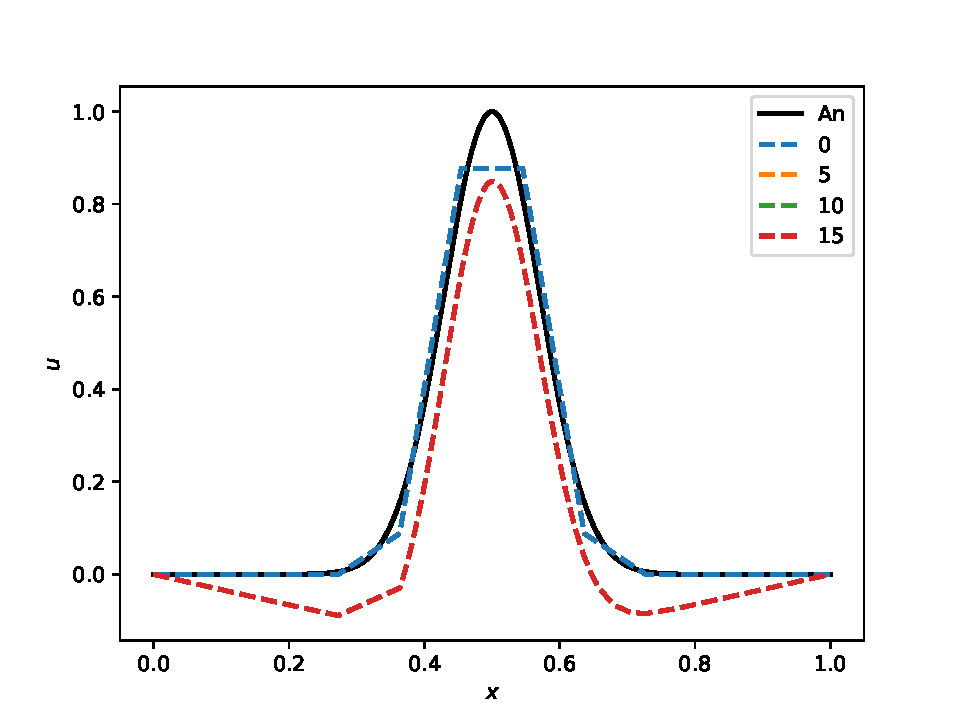
\includegraphics[width=0.85\linewidth]{plots/solutionTask1dAMRFirst.pdf}}\hspace{0mm}
\subfloat[\textbf{AMR second order}]{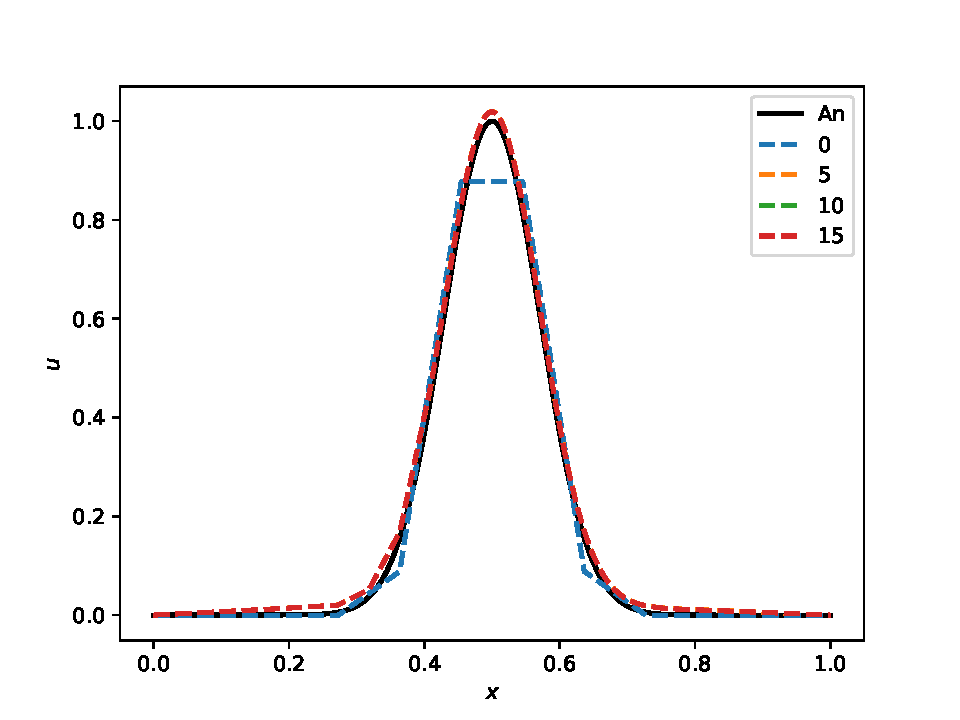
\includegraphics[width=0.85\linewidth]{plots/solutionTask1dAMRSecond.pdf}}\hspace{0mm}
\caption{Poisson equation with manufactured solution $u(x) = \exp{\left(-\frac{1}{\epsilon}(x-\frac{1}{2})^2\right)}$, with Dirichlet boundary conditions $u(0) = u(1) = \exp{\left(-\frac{1}{4\epsilon}\right)}$.  The numerical solution is computed with \textbf{AMR}, combined with a  \textbf{first order method} (a) and \textbf{second order method} (b). The integers in the legend refer to the number of iterations in the refinement, i.e. 15 refers to a solution where the grid maximally has been adaptively refined 15 times, depending on if the chosen criterion is met. The initial grid  has $M = 10$ points.}
\label{fig:part1Task1dSolutionAMR}
\end{figure}

\begin{figure}[t]
\centering
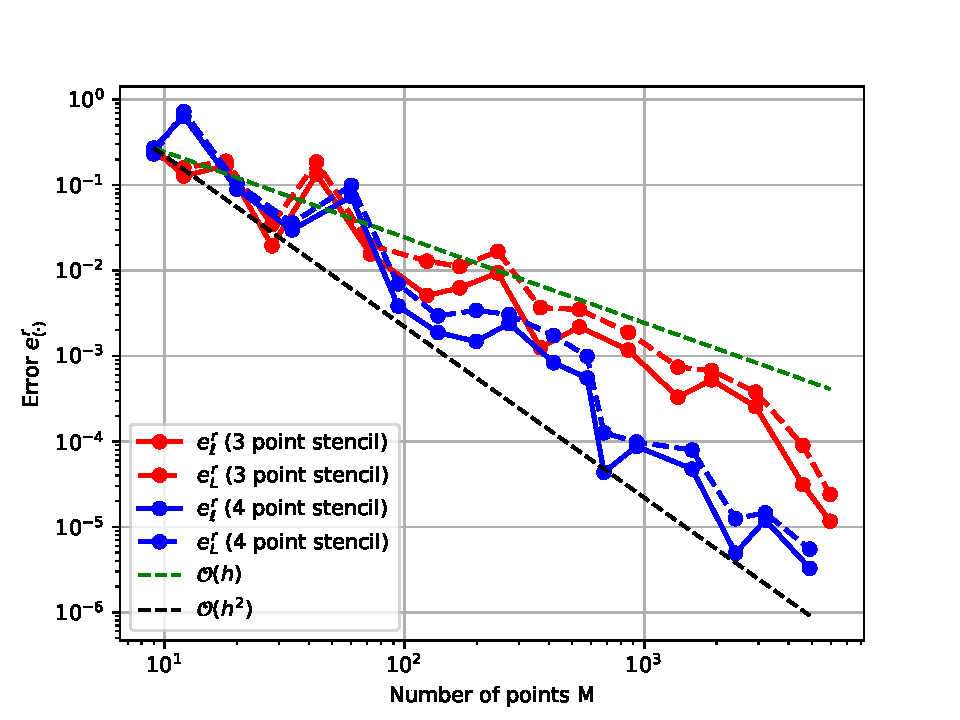
\includegraphics[width=0.85\linewidth]{plots/loglogtask1dAMR.pdf}
\caption{Poisson equation with manufactured solution $u(x) = \exp{\left(-\frac{1}{\epsilon}(x-\frac{1}{2})^2\right)}$, with Dirichlet boundary conditions $u(0) = u(1) = \exp{\left(-\frac{1}{4\epsilon}\right)}$. The graph depicts a "log-log" plot of relative errors when $h \rightarrow 0$, when solving the problem using \textbf{AMR}. First and second order functions of $h$ are added in order to compare the convergence of the numerical solution to the theoretical results.}
\label{fig:part1Task1dloglogAMR}
\end{figure}


\newpage
\ 
\newpage
